\documentclass[11pt]{beamer}
\usetheme{Madrid}
\usefonttheme{serif}

\usepackage[utf8]{inputenc}
\usepackage[vietnamese]{babel}
\usepackage[T5]{fontenc}

\usepackage{amsmath}
\usepackage{amsfonts}
\usepackage{amssymb}
\usepackage{graphicx}

\DeclareMathOperator{\sen}{sen}
\DeclareMathOperator{\tg}{tg}

\setbeamertemplate{caption}[numbered]

\author[University of Information Technology]{Thành viên thực hiện: \\ Hà Thanh Phong - 24520024 \\ Hà Xuân Thiện - 24520031 \\ Trần Quang Trường - 24521901}
\title[Chaper 18]{Context-Free Grammars and Constituency Parsing}
\newcommand{\email}{email}
\setbeamertemplate{navigation symbols}{} 
\institute[]{University of Information Technology - VNUHCM} 
\date{\today} 
\bibliographystyle{apalike}

\usepackage{tikz}
\usetikzlibrary{positioning,arrows.meta,calc}
\usepackage{amsmath}
\usepackage{caption}

\tikzset{
	img/.style={draw=black, line width=1pt, inner sep=0pt},
	state/.style={circle, draw=black, line width=1.4pt, minimum size=12mm, text=black, font=\Large},
	darr/.style={draw=black, line width=1.4pt, -{Latex[length=4mm,width=3mm]}},
	dlink/.style={draw=black, line width=1.2pt, dashed},
	txt/.style={text=black, font=\Large}
}
\usepackage{graphicx}
\usepackage{animate}
\usepackage{tikz}
\usetikzlibrary{calc}



\usepackage{amsmath}
\usetikzlibrary{arrows.meta,positioning}

\begin{document}
	
	\begin{frame}
		\titlepage
	\end{frame}
	
	\begin{frame}{Mục lục}
		\tableofcontents[hideallsubsections]
	\end{frame}


	\section{CKY Parsing: A Dynamic Programming Approach}
	\begin{frame}{Mục lục}
		\tableofcontents[currentsection]
	\end{frame}

	\begin{frame}{18.6 CKY Parsing: A Dynamic Programming Approach}
		\begin{block}{Khái niệm}
			CKY (Cocke-Kasami-Younger) là thuật toán parsing dựa trên \textbf{quy hoạch động (dynamic programming)}.
		\end{block}
		\begin{itemize}
			\item \textbf{Ý tưởng chính:} Thay vì phân tích lại cùng một cụm nhiều lần, ta lưu kết quả của các đoạn nhỏ vào một bảng để xây dựng các đoạn lớn hơn.
		\end{itemize}
	\end{frame}
	
	\begin{frame}{18.6.1. Conversion to Chomsky Normal Form}
		
		Để sử dụng CKY, ngữ pháp (grammar) phải được chuyển sang \textbf{Chomsky Normal Form (CNF)}.
		\vspace{0.3cm}
		
		\begin{block}{Quy tắc Grammar trong CNF}
			Grammar trong CNF tuân theo một trong 2 kiểu sau:
			\begin{itemize}
				\item $A \rightarrow B\ C$
				\item $A \rightarrow w$
			\end{itemize}
		\end{block}
		
	\end{frame}

	\begin{frame}{18.6.1. Conversion to Chomsky Normal Form}
		\textbf{Các rule cần xử lý khi chuyển sang CNF:} 
		\begin{enumerate}
			\item Trộn terminal và non-terminal ở vế phải.
			\item Unit production ($A \rightarrow B$).
			\item Vế phải dài hơn 2 symbol ($A \rightarrow B \ C \ D$).
		\end{enumerate}
	\end{frame}
	
	\begin{frame}{18.6.1. Conversion to Chomsky Normal Form}
		\textbf{Cách xử lý các rule:}
		
		\begin{itemize}
			\item \textbf{Trộn Terminal và Non-terminal:} \\ Tạo một dummy non-terminal mới.
			\begin{itemize}
				\item \textit{Ví dụ:} \texttt{INF-VP $\rightarrow$ to VP} 
				\item \textit{Đổi thành:} \texttt{INF-VP $\rightarrow$ TO VP} và \texttt{TO $\rightarrow$ to}
			\end{itemize}
			
			\pause
			\vfill
			
			\item \textbf{Unit Production ($A \rightarrow B$):} \\ Loại bỏ role trung gian, thay A bằng các rule thật mà B có thể sinh ra.
			\begin{itemize}
				\item \textit{Cách làm:} Nếu có chuỗi $A \rightarrow B$ và $B \rightarrow \beta$, ta thêm quy tắc \texttt{$A \rightarrow \beta$} và loại bỏ quy tắc trung gian.
			\end{itemize}
			
			\pause
			\vfill
			
			\item \textbf{Quy tắc dài hơn 2 symbol:} \\ Tách thành các cặp nhị phân bằng cách sử dụng các biến trung gian ($X, Y \dots$).
			\begin{itemize}
				\item \textit{Ví dụ:} \texttt{A $\rightarrow$ B C D}
				\item \textit{Đổi thành:} \texttt{A $\rightarrow$ B X} và \texttt{X $\rightarrow$ C D}
			\end{itemize}
		\end{itemize}
	\end{frame}

	\begin{frame}{18.6.1. Conversion to Chomsky Normal Form}
		\begin{figure}
			\centering
			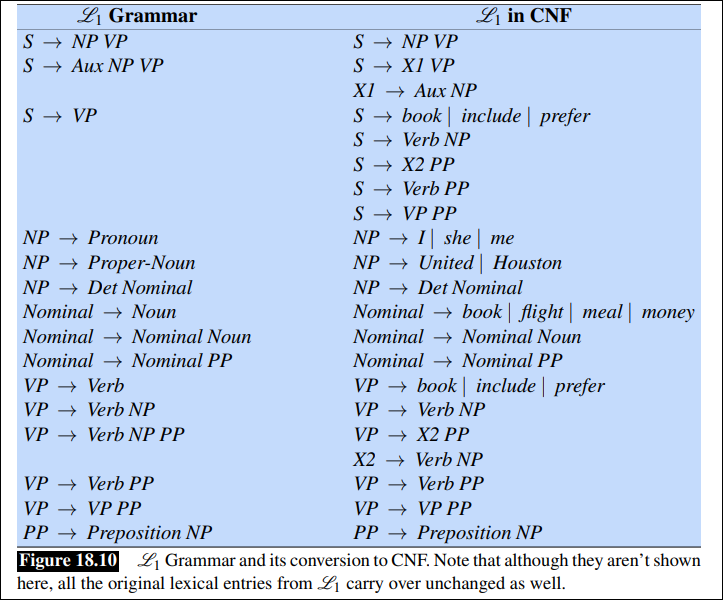
\includegraphics[width=0.75\linewidth]{18.10}
		\end{figure}
	\end{frame}
	
	
	\begin{frame}{18.6.2 CKY Recognition}
		\textbf{Thuật toán CKY:}
		\begin{itemize}
			\item Thuật toán thực hiện trên ma trận tam giác $[0 \dots n, 0 \dots n]$.
			\item Mỗi ô $[i, j]$ lưu các non-terminal có thể bao phủ từ vị trí $i$ đến $j$.
			
			\item Để tìm ô $[i, j]$, thuật toán tìm điểm cắt $k$ sao cho thỏa mãn:
			$$A \rightarrow B \ C $$
			Trong đó $B \in \text{ô } [i, k]$ (bên trái) và $C \in \text{ô } [k, j]$ (bên dưới).
			
			\item Một câu được Grammar chấp nhận khi ô [0, n] chứa $S$.
		\end{itemize}
	\end{frame}
	
	
	\begin{frame}{18.6.2 CKY Recognition}
		\begin{figure}
			\centering
			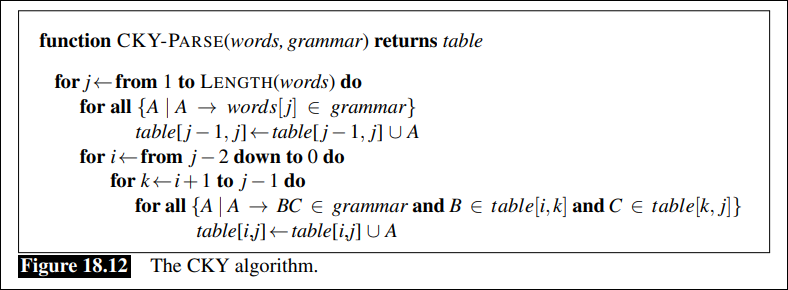
\includegraphics[width=1\linewidth]{18.12}
		\end{figure}
	\end{frame}	
	\begin{frame}{18.6.2 CKY Recognition}
		\begin{figure}
			\centering
			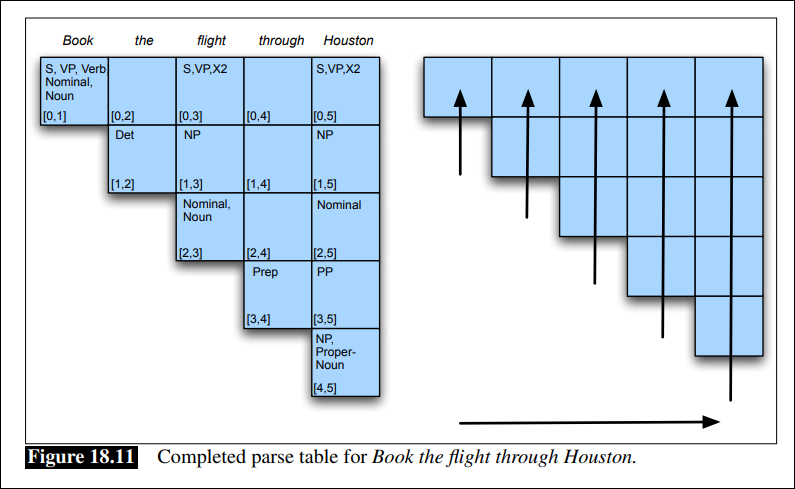
\includegraphics[width=1\linewidth]{18.11}
		\end{figure}
	\end{frame}	
	
	\begin{frame}{18.6.3 CKY Parsing}
		
		Thuật toán vừa đề cập chỉ cho ta biết câu được cho có parse được hay không, chứ chưa trả về Parse tree.
		
		\vspace{0.5cm}
		Để trả về Parse tree, ta cần:
		\begin{itemize}
			\item \textbf{Bổ sung Backpointers:} Mỗi non-terminal trong bảng được lưu kèm với các con trỏ dẫn đến các mục (entries) đã tạo ra nó.
			\item \textbf{Chấp nhận đa phiên bản:} Cho phép lưu trữ nhiều phiên bản của cùng một non-terminal trong cùng một ô nếu chúng có nguồn gốc dẫn xuất khác nhau.
		\end{itemize}

	\end{frame}
	
	\begin{frame}{18.6.3 CKY Parsing}
		\textbf{Quá trình tạo Parse Tree:}
		\begin{itemize}
			\item Bắt đầu từ nhãn $S$ tại ô $[0, n]$, ta \textbf{đệ quy} xuống các thành phần con thông qua các con trỏ để dựng lại toàn bộ cây.
			\item Bảng CKY lúc này chứa đựng \textbf{tất cả} các cách phân tích khả dĩ cho câu đầu vào.
			\item Tuy nhiên, trên thực tế, thay vì lấy \textbf{mọi cây}, ta cần tìm cây "tốt nhất" (Best Parse) thông qua các mô hình xác suất.
		\end{itemize}
	\end{frame}
	
	\begin{frame}{18.6.3 CKY Parsing}
		\begin{columns}
			\column{0.4\textwidth}
			\begin{figure}
				\centering
				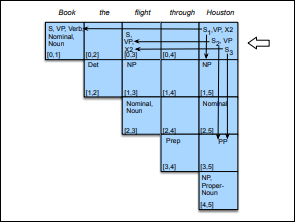
\includegraphics[width=1\linewidth]{18.14.2}
				\caption*{Figure 18.14. Filling the cells of column 5 after reading the word Houston}
			\end{figure}
	        \column{0.6\textwidth}
			\begin{figure}
				\centering
				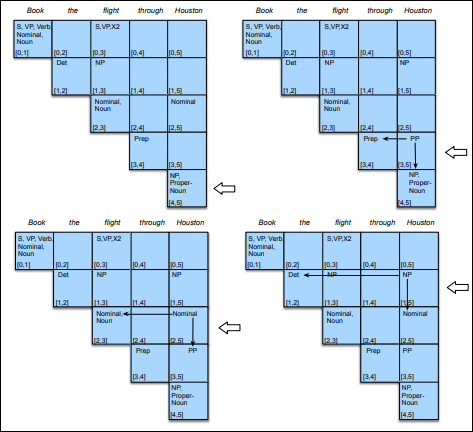
\includegraphics[width=1\linewidth]{18.14.1}
			\end{figure}
		\end{columns}

	\end{frame}
	

	\begin{frame}{18.6.4 CKY in Practice}
		\textbf{Trên thực tế}, CNF có thể làm parse tree khác với cây gốc mà người thiết kế grammar mong muốn.
		
		\vspace{0.5cm}
		Ví dụ: 
		\begin{itemize}
			\item Khi một rule dài bị tách thành nhiều rule nhị phân, cây parse sẽ xuất hiện thêm các \textbf{dummy non-terminal}.
			\item Những node giả này có ích cho thuật toán, nhưng có thể \textbf{gây khó khăn} nếu ta muốn dùng parse tree cho semantic analysis.
		\end{itemize}
		
	\end{frame}
	
	\begin{frame}{18.6.4 CKY in Practice}
		\textbf{Khôi phục parse tree gốc (Post-processing):}
		
		\begin{itemize}
			\item \textbf{Xử lý nút giả:} \\
			Bằng cách xóa các nút trung gian và đẩy các con trực tiếp của nó lên lại nút cha ban đầu.
			\vspace{0.5cm}
			\item \textbf{Xử lý Unit Productions:} \\
			Chỉnh sửa trực tiếp thuật toán CKY để  xử lý unit production trực tiếp thay vì loại bỏ hoàn toàn.
			
		\end{itemize}
	\end{frame}
	
	\section{Span-Based Neural Constituency Parsing}
	\begin{frame}{Mục lục}
		\tableofcontents[currentsection]
	\end{frame}
	
	\begin{frame}{18.7 Span-Based Neural Constituency Parsing}
		\begin{block}{Vấn đề của CKY truyền thống}
			CKY liệt kê được mọi cây parse nhưng \textbf{thiếu khả năng} để chọn ra cây đúng nhất.
		\end{block}
		
		\vfill
		Ý tưởng của \textbf{Span-Based Neural Parsing} (hay Neural CKY):
		\begin{itemize}
			\item Thay vì rule thủ công, ta dùng một \textbf{Neural Classifier} để gán điểm số (\textit{score}) cho từng span có nhãn.
			\item Sử dụng biến thể CKY để tìm cây có \textbf{tổng score cao nhất}.
		\end{itemize}

	\end{frame}
	
	\begin{frame}{18.7.1 Computing Scores for a Span}
		
		$score s(i, j, l)$ là điểm cho giả thuyết rằng đoạn từ $i$ đến $j$ là một constituent loại $l$.
		\vspace{0.5cm}
		
		Để tính $score s(i, j, l)$, ta thực hiện các bước sau:
		\begin{itemize}
			\item Đưa câu vào mô hình ngôn ngữ.
			\item Đầu ra của mô hình cần được đưa về \textbf{word representation}.
			\item Các \textbf{word representation} này có thể được đưa qua thêm một số postprocessing layer.
			\item Sau đó, mô hình tạo \textbf{representation} cho từng span dựa trên hai đầu mút của span.
		\end{itemize}
	\end{frame}
	\begin{frame}{18.7.1 Computing Scores for a Span}
		\begin{figure}
			\centering
			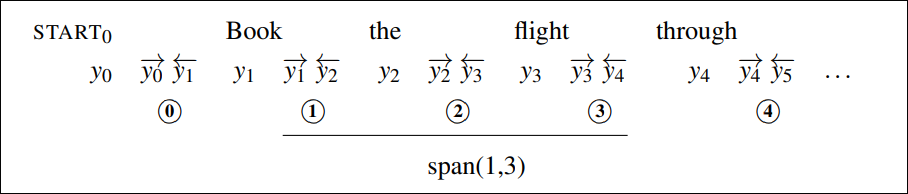
\includegraphics[width=1\linewidth]{image-01}
		\end{figure}
		
		\pause
		\textbf{Span representation} thường được tạo bằng cách lấy hiệu giữa embedding ở điểm kết thúc và điểm bắt đầu:
		\begin{equation}
			v(i, j) = [\vec{y_j} - \vec{y_i} \ ; \ \overleftarrow{y_{j+1}} - \overleftarrow{y_{i+1}}]
			\tag{18.5}
		\end{equation}

	\end{frame}
	
	\begin{frame}{18.7.1 Computing Scores for a Span}
		\textbf{Span representation} thường được tạo bằng cách lấy hiệu giữa embedding ở điểm kết thúc và điểm bắt đầu:
		\begin{equation}
			v(i, j) = [\vec{y_j} - \vec{y_i} \ ; \ \overleftarrow{y_{j+1}} - \overleftarrow{y_{i+1}}]
			\tag{18.5}
		\end{equation}
		
		\vspace{0.5cm}
		
		Sau khi có vector \textbf{span representation}, mô hình đưa vector này qua một MLP để sinh ra score cho từng non-terminal label có thể có. 
		\begin{equation}
			s(i, j, \cdot) = \mathbf{W}_2 \text{ ReLU}(\text{LayerNorm}(\mathbf{W}_1 \mathbf{v}(i, j)))
			\tag{18.6}
		\end{equation}
	\end{frame}
	
	\begin{frame}{18.7.1 Computing Scores for a Span}
		\begin{figure}
			\centering
			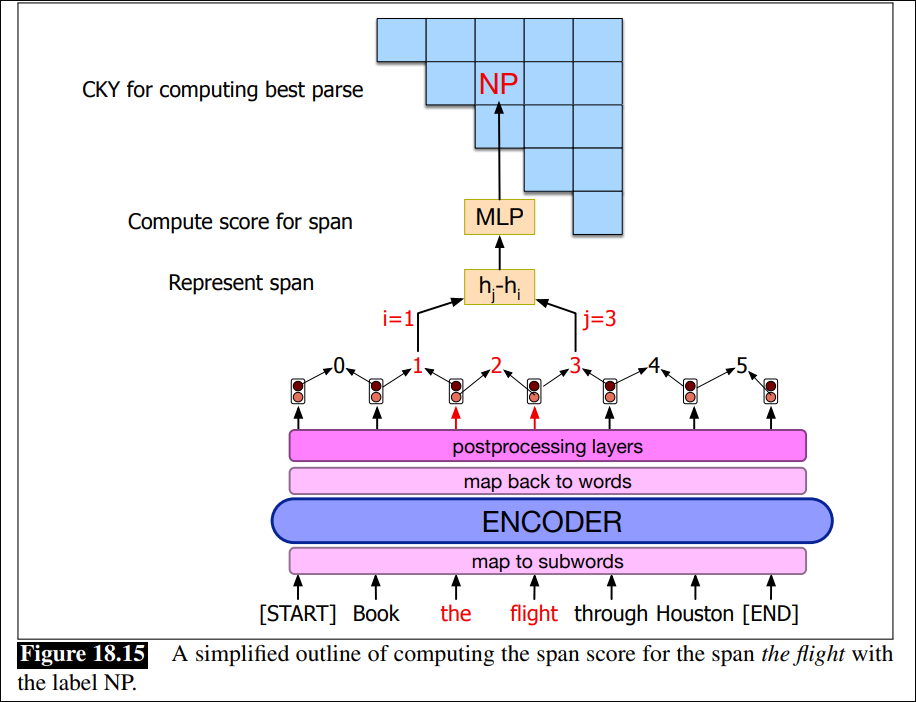
\includegraphics[width=0.8\linewidth]{18.15}
		\end{figure}
	\end{frame}
	
	\begin{frame}{18.7.2 Integrating Span Scores into a Parse}
		Gọi cây $T$ là tập gồm $|T|$ span, với span thứ $t^{th}$ bắt đầu từ $i_t$ kết thúc tại $j_t$, với loại $l_t$:
			\begin{equation}
				T = \{ (i_t, j_t, l_t) : t = 1, \ldots, |T|\}
				\tag{18.7}
			\end{equation}
		
		\pause
		Score của cả cây $s(T)$ bằng tổng score của tất cả span trong cây:
			\begin{equation}
				s(T) = \sum_{(i, j, l) \in T} s(i, j, l)
				\tag{18.8}
			\end{equation}
		\pause
		
		Cuối cùng, ta chọn parse tree với điểm số lớn nhất:
			\begin{equation}
				\hat{T} = \mathop{\text{argmax}}_{T} s(T) 
				\tag{18.9}
			\end{equation}
	\end{frame}
	
	\begin{frame}{18.7.2 Integrating Span Scores into a Parse}
		\textbf{Cách tiếp cận:} Lựa chọn nhãn có score cao nhất $s(i, j, l)$ cho từng span.
		\vspace{0.5cm}
		
		$\rightarrow$ Cách tiếp cận này \textbf{không đảm bảo} các span được chọn sẽ tạo thành một cây hợp lệ.
		\vspace{0.5cm}
		
		$\rightarrow$ Trong thực tế, người ta sử dụng một biến thể của CKY để tìm cây có \textbf{tổng score tốt nhất}.

	\end{frame}
	
	\begin{frame}{18.7.2 Integrating Span Scores into a Parse}
		
		Gọi $s_{best}(i, j)$ là điểm của subtree span $(i, j)$ tốt nhất.
		
		\vspace{0.5cm}
		Với span có độ dài bằng $1$:
		\begin{equation}
			s_{\text{best}}(i, i+1) = \max_{l} s(i, i+1, l) 
			\tag{18.10}
		\end{equation}
		
		Với span còn lại, ta gọi đệ quy:
		\begin{equation}
		\begin{aligned}
			s_{\text{best}}(i, j) &= \max_{l} s(i, j, l) \\
			&+ \max_{k} [s_{\text{best}}(i, k) 
			+ s_{\text{best}}(k, j)] 
		\end{aligned}
\tag{18.11}
		\end{equation}

	\end{frame}
	
	
	\section{Evaluating Parsers}
	\begin{frame}{Mục lục}
		\tableofcontents[currentsection]
	\end{frame}
	\begin{frame}{18.8 Evaluating Parsers}
		\begin{itemize}
			\item Parser thường được đánh giá bằng PARSEVAL metrics.
			
			\item Ý tưởng của PARSEVAL là so sánh parse tree do model dự đoán với gold parse tree.
			
			\item Một \textbf{constituent} trong hypothesis parse \textbf{được xem là đúng} nếu nó khớp với constituent trong reference parse ở ba điểm:
			\begin{itemize}
			\item Cùng vị trí bắt đầu.
			\item Cùng vị trí kết thúc.
			\item Cùng non-terminal label.
			\end{itemize}
		\end{itemize}
	\end{frame}
	
	\begin{frame}{18.8 Evaluating Parsers}
		Từ đó, ta có hai metric chính:
	\begin{itemize}
		\item labeled recall = $\frac{\text{\# of correct constituents in hypothesis parse of } s}{\text{\# of total constituents in reference parse of } s}$
		
		\vspace{0.5cm}
		
		\item labeled precision = $\frac{\text{\# of correct constituents in hypothesis parse of } s}{\text{\# of total constituents in hypothesis parse of } s}$
	\end{itemize}
		\pause
		\vspace{0.5cm}
		Ta có thể gộp cả precision và recall thành F1:
		\begin{equation}
			F1 = \frac{2PR}{P + R}
			\tag{18.12}
		\end{equation}
	\end{frame}

	\section{Heads and Head-Finding}
	\begin{frame}{Mục lục}
		\tableofcontents[currentsection]
	\end{frame}
	
	\begin{frame}{18.9 Heads and Head-Finding}
		\begin{block}{Head}
			Mỗi thành phần cú pháp (constituent) đều gắn liền với một từ quan trọng nhất về mặt ngữ pháp, gọi là \textbf{head}.
			\begin{itemize}
				\item Danh từ (N) là head của cụm danh từ (NP).
				\item Động từ (V) là head của cụm động từ (VP).
			\end{itemize}
			
			Head rất quan trọng vì nó giúp liên kết \textbf{constituency parsing} với \textbf{dependency parsing}.
		\end{block}
		\pause
		\begin{block}{Head-Finding}
		Nếu \textbf{constituency parser} cho ta cấu trúc phrase, thì head-finding giúp xác định \textbf{từ trung tâm} của mỗi phrase, từ đó có thể chuyển sang \textbf{quan hệ phụ thuộc} giữa các từ.
		\end{block}
		
	\end{frame}
	
	\begin{frame}{18.9 Heads and Head-Finding}
		\begin{figure}
			\centering
			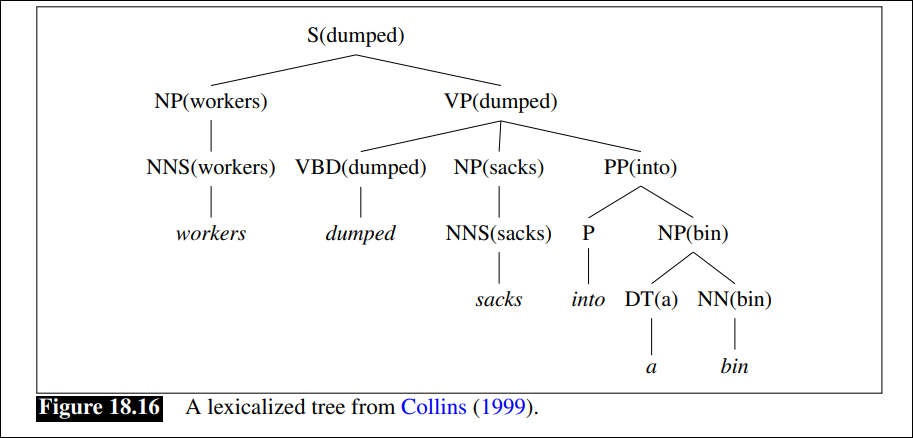
\includegraphics[width=1\linewidth]{18.16}
		\end{figure}
	\end{frame}
	
	\begin{frame}{18.9 Heads and Head-Finding}
		\begin{itemize}
		\item Trong thực tế, \textbf{việc chọn head} không phải lúc nào cũng rõ ràng. 
		
		\vspace{0.5cm}
		\item Vì vậy, nhiều hệ thống dùng \textbf{head rules viết tay}. 
				
		\vspace{0.5cm}
				
		\item Các rule này duyệt qua con của một node theo \textbf{thứ tự ưu tiên} để tìm head. 
		\end{itemize}
	\end{frame}
	
	\begin{frame}{18.9 Heads and Head-Finding}
		Ví dụ với NP, hệ thống có thể tìm từ phải sang trái để xem có noun tag như NN, NNP, NNPS hay không; nếu có thì chọn nó làm head.
		
		\begin{figure}
			\centering
			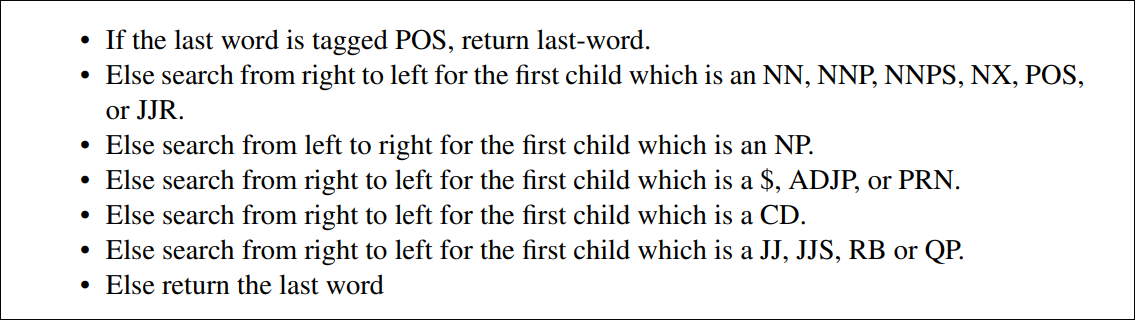
\includegraphics[width=1\linewidth]{image-02}
		\end{figure}
		
		\pause
		$\rightarrow$ Các head rules như vậy còn được gọi là \textbf{head percolation table}, vì head được truyền dần từ các node con lên node cha trong parse tree.
	\end{frame}
		
	\begin{frame}{18.9 Heads and Head-Finding}
		\begin{figure}
			\centering
			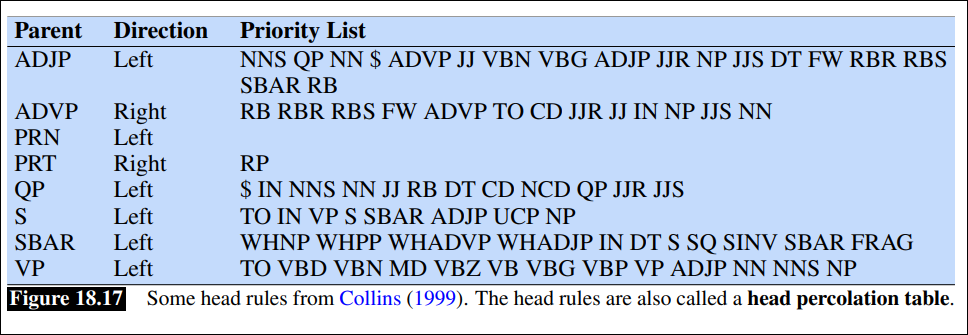
\includegraphics[width=1\linewidth]{18.17}
		\end{figure}
	\end{frame}
\end{document}